\documentclass[tikz]{standalone}

\usetikzlibrary{decorations.pathreplacing,
  decorations.markings,
  decorations.pathmorphing}
 \usetikzlibrary{patterns}
\usetikzlibrary{arrows}
\usetikzlibrary{arrows.meta}
\usetikzlibrary{shapes.misc}


\begin{document}
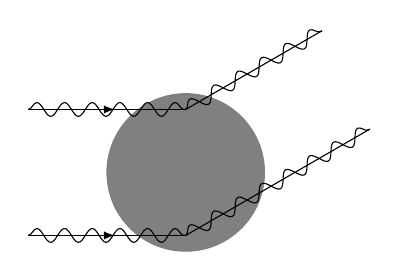
\begin{tikzpicture}
\draw[gray,fill=gray] (0,0) circle (1);
\draw[decorate, decoration={snake}] (-2,0.8) -- (0,0.8);
\draw[decorate, decoration={snake}] (-2,-0.8) -- (0,-0.8);
\draw[decorate, decoration={snake}] (0,0.8) -- ++(30:2);
\draw[decorate, decoration={snake}] (0,-0.8) -- ++(30:2.7);
\draw[postaction={decorate,decoration={markings,mark=at position .55 with {\arrow{latex}}}}] (-2,0.8) -- (0,0.8);
\draw[postaction={decorate,decoration={markings,mark=at position .55 with {\arrow{latex}}}}] (-2,-0.8) -- (0,-0.8);
\draw (0,0.8) -- ++(30:2);
\draw (0,-0.8) -- ++(30:2.7);
\end{tikzpicture}
\end{document}
